\documentclass[12pt]{article}
\usepackage{epsf}
\usepackage{amssymb}
\usepackage{enumitem}
\usepackage{amsmath}
\usepackage{tikz}
\usetikzlibrary{automata, positioning, arrows, petri}

\title{aashlock-331-hw8}
\author{Aren Ashlock}
\date{March 26, 2024}

\setlength{\oddsidemargin}{-0.25in}
\setlength{\topmargin}{-0.5in}
\setlength{\headheight}{0cm}
\setlength{\headsep}{0cm}
\setlength{\textheight}{10in}
\setlength{\textwidth}{7in}
\setlength{\topskip}{0cm}

\begin{document}

\noindent\textbf{ComS 331 \quad Spring 2024 \quad Name: Aren Ashlock}

\begin{enumerate}

%----------------------------------- Q1 DONE -----------------------------------

\item We know that NPDA can sum: $L = \{a^ib^jc^{i+j} : i,j \in \mathbb{N}\}$ is a CFL. Petri nets can perform the same operation: show a T-type Petri net for the same language.

\begin{tikzpicture}
    [node distance = 1.5cm]

    % letter tansitions
    \node[place, label=left:$p_1$, tokens=1] (p1){};
    \node[transition, below of=p1, label=left:$t_1$] (t1) {$\epsilon$}
        edge[pre] (p1);
    \node[place, label=left:$p_2$, below of=t1] (p2){}
        edge[pre] (t1);
    \node[transition, above right of=p2, label=above:$t_2$] (t2) {$\epsilon$}
        edge[pre] (p2);
    \node[place, label=above:$p_3$, right of=t2] (p3){}
        edge[pre] (t2);

    % counting letters
    \node[transition, right of=p1, label=above:$t_3$] (t3) {$a$}
        edge[pre, bend left = 20] (p1)
        edge[post, bend right = 20] (p1);
    \node[place, label=above:$p_4$, right of=t3] (p4){}
        edge[pre] (t3);
    \node[transition, right of=p2, label=below:$t_4$] (t4) {$b$}
        edge[pre, bend left = 20] (p2)
        edge[post, bend right = 20] (p2);
    \node[place, label=below:$p_5$, right of=t4] (p5){}
        edge[pre] (t4);

    \node[transition, below right of=p4, label=above:$t_5$] (t5) {$c$}
        edge[pre] (p4)
        edge[pre, bend right = 20] (p3)
        edge[post, bend left = 20] (p3);
    \node[transition, right of=p5, label=above:$t_6$] (t6) {$c$}
        edge[pre] (p5)
        edge[pre, bend left = 10] (p3)
        edge[post, bend right = 10] (p3);
    
\end{tikzpicture}

%-------------------------------------------------------------------------------

%----------------------------------- Q2 DONE -----------------------------------

\item Consider the language $L = \{w \in \{a,b,c\}^* : |w|_a = |w|_b = |w|_c\}$.

\begin{enumerate}[label=(\alph*)]

%----------------------------------- Q2A DONE ----------------------------------
    
    \item Prove that $L$ is not a context-free language.

    \color{blue}
        Let $L$ be a CFL. Then, $\exists m, \forall |w| \geq m, \exists uvxyz = w, |vy| > 0, |vxy| \leq m, \exists k, uv^kxy^kz \in L$. Let's have $w$ where $|w|_a = |w|_b = |w|_c = m$. We can break it down into 2 cases...

        \textbf{Case 1:} $v$ and $y$ only consist of 1 type of letter ($a, b, c$). Choosing to pump with $k = 0$, we get any of these 3 results: (1) $|w|_a = m-i-j$, (2) $|w|_b = m-i-j$, (3) $|w|_c = m-i-j$. In all 3 results, the number of $a$'s, $b$'c, and $c$'s are not equal. Thus, $w \notin L$.

        \textbf{Case 2:} $v$ and $y$ consist of 2 types of letters ((1) $a$ and $b$, (2) $b$ and $c$, or (3) $a$ and $c$). Choosing to pump with $k = 0$, we get these 3 results: (1) $|w|_a = m-i$ AND $|w|_b = m-j$, (2) $|w|_b = m-i$ AND $|w|_c = m-j$, (3) $|w|_a = m-i$ AND $|w|_c = m-j$. In all 3 results, the number of $a$'s, $b$'c, and $c$'s are not equal since at least $i > 1$ or $j > 1$. Thus, $w \notin L$.

        Since $|vxy| \leq m$, it is \textbf{impossible} for $v$ and $y$ \textbf{to consist of all 3 types of letters}.

        It's evident that there are no cases where $w$ can be pumped, therefore, $L$ \textbf{is not context-free}.
    \color{black}

%-------------------------------------------------------------------------------

%----------------------------------- Q2B DONE ----------------------------------
    
    \item Prove that $L$ is an L-type non-$\epsilon$ labeling Petri net language.

    \color{red}
        I have no clue and spent too much time trying to figure this out. At least I don't loose any points...
    \color{black}

%-------------------------------------------------------------------------------

%----------------------------------- Q2C DONE ----------------------------------
    
    \item Prove that $L$ is a T-type unrestricted labeling Petri net language.

    \begin{tikzpicture}
        [node distance = 2cm]
    
        % letter tansitions
        \node[place, label=below:$p_1$, tokens=1] (p1){};
        \node[transition, left of=p1, label=below:$t_1$] (t1) {$\epsilon$}
            edge[pre, bend left = 20] (p1)
            edge[post, bend right = 20] (p1);
        \node[transition, right of=p1, label=below:$t_2$] (t2) {$\epsilon$}
            edge[pre] (p1);
        \node[place, right of=t2, label=below:$p_5$] (p5) {}
            edge[pre] (t2);

        \node[place, above left of=p1, label=below right:$p_2$] (p2) {}
            edge[pre] (t1);
        \node[place, above of=p2, label=below right:$p_3$] (p3) {}
            edge[pre, bend right = 20] (t1);
        \node[place, below left of=p1, label=below:$p_4$] (p4) {}
            edge[pre] (t1);

        \node[transition, above right of=p5, label=above left:$t_3$] (t3) {$b$}
            edge[pre] (p2)
            edge[pre, bend right = 20] (p5)
            edge[post, bend left = 10] (p5);
        \node[transition, above right of=t3, label=above left:$t_4$] (t4) {$a$}
            edge[pre] (p3)
            edge[pre, bend left = 20] (p5)
            edge[post, bend left = 40] (p5);
        \node[transition, below right of=p5, label=below left:$t_5$] (t5) {$c$}
            edge[pre] (p4)
            edge[pre, bend left = 20] (p5)
            edge[post, bend right = 20] (p5);
        
        
    \end{tikzpicture}

    \color{blue}
        Here is a T-type unrestricted labeling Petri net that accepts $L$. This \textbf{proves} that $L$ is a T-type unrestricted labeling Petri net language.
    \color{black}

%-------------------------------------------------------------------------------

\end{enumerate}
\end{enumerate}
\end{document}